\documentclass[11pt]{metabo}

\usepackage[font={small}]{caption}
\usepackage{natbib}
\usepackage{graphicx, graphics, subfigure, multirow}
\usepackage{envmath, amssymb}
\everymath{\displaystyle}
\usepackage{fancyhdr, lscape}
\usepackage{pgf,tikz}
\usetikzlibrary{shapes}
\usepackage{pstricks}
\usepackage{lmodern}
\usepackage{pifont}
\usepackage{comment}
\usepackage{yfonts}

\renewcommand{\labelitemi}{$\bullet$}
\renewcommand{\labelitemii}{$\cdot$}
\renewcommand{\labelitemiii}{$\diamond$}
\renewcommand{\labelitemiv}{$\ast$}

\newcommand{\J}{\textswab{J}}
\newcommand{\p}{\partial}
\newcommand{\RA}{\Rightarrow}
\newcommand{\LA}{\Leftarrow}



\title{\bsc{Réseaux métaboliques}\\  \textit{de Daniel Kahn}}
\author{Simon B.G. \& Virginie J.}
%\date{}

\begin{document}

\maketitle
\tableofcontents

\newpage
\renewcommand{\labelitemi}{$\bullet$}
\renewcommand{\labelitemii}{$\cdot$}
\renewcommand{\labelitemiii}{$\diamond$}
\renewcommand{\labelitemiv}{$\ast$}

\section{Introduction sur le métabolisme \& remise à niveau en enzymologie}

\paragraph{Objectif général de ce cours}
\begin{itemize}
    \item[$\bullet$] Comprendre le comportement général des systèmes métaboliques
    \item Aptitude à modéliser leurs dynamiques
    \item Exprimer comment les propriétés cinétiques des enzymes affecte les concentrations en métabolites et les flux
    \item Examiner comment les données expérimentales peuvent être utiliser pour identifier un modèle métabolique
    \item Interpréter ces comportements en terme de régulation biologique
    \item Généraliser au réseau de transcription des signaux
\end{itemize}

\paragraph{Pré-requis}
\begin{itemize}
    \item Connaissance sur la cinétique enzymatique
    \item Algèbre linéaire : 
    \begin{itemize}
    	\item Analyse de rang matriciel, diagonalisation, etc ...
        \item Etre familier avec les packages mathématiques comme Scilab, Maple, R ou Matlab
    \end{itemize}
    \item Système Dynamique
    \begin{itemize}
        \item Jacobienne
        \item Analyse de stabilité
    \end{itemize}
\end{itemize}

\paragraph{Outline}
\begin{enumerate}
    \item Introduction sur le métabolisme
    \item Méthode pour étudier le métabolisme
    \item Remise à niveau en cinétique enzymatique
\end{enumerate}



\subsection {Qu'est-ce que le métabolisme ?}
\begin{itemize}
    \item Usine du vivant de produits chimiques : typiquement plusieurs centaines de réactions impliquant de petites molécules 
    \item Balances
        \begin{itemize}
            \item Nutriments et produits
            \item Energie
            \item Produit du pouvroi réducteur (redox)
        \end{itemize}
    \item Turn-over rapide
    \item Les réactions chimiques souvent catalyser par des enzymes
\end{itemize} 


\begin{figure}
    \centering
    \begin{tabular}{cc}
        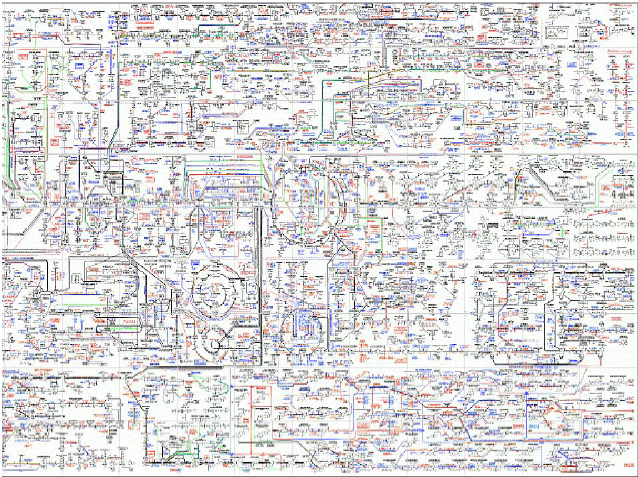
\includegraphics[width =8 cm]{Images/1.PNG} & 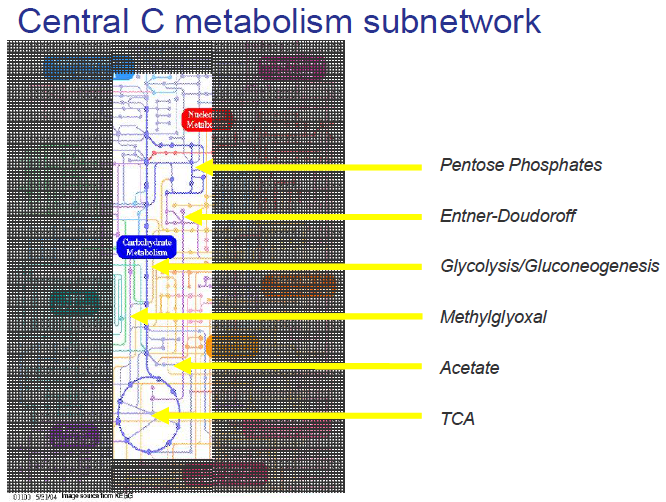
\includegraphics[width =8 cm]{Images/2.PNG} \\
        \textit{Métabolisme} & \textit{Central C metabolism subnetwork} \\
        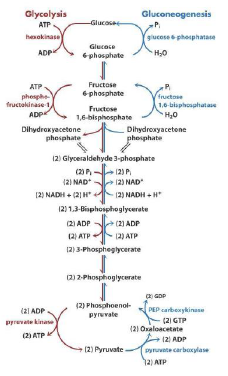
\includegraphics[width =8 cm]{Images/3.PNG} & 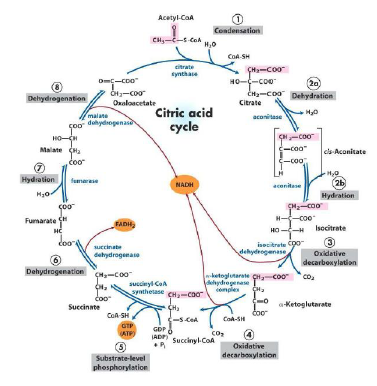
\includegraphics[width =8 cm]{Images/4.PNG} \\
        \textit{Glycolyse et néoglucogénèse}   &   \textit{TCA cycle} \\
    \end{tabular}
\end{figure}

\begin{figure}
    \centering
    \begin{tabular}{cc}
        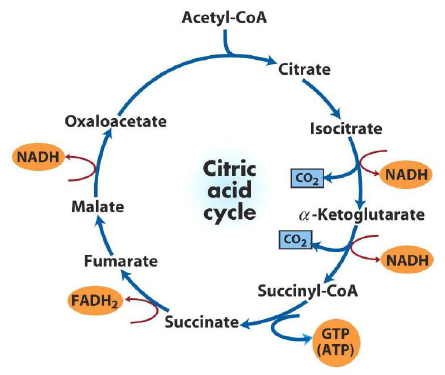
\includegraphics[width =8 cm]{Images/5.PNG}    &   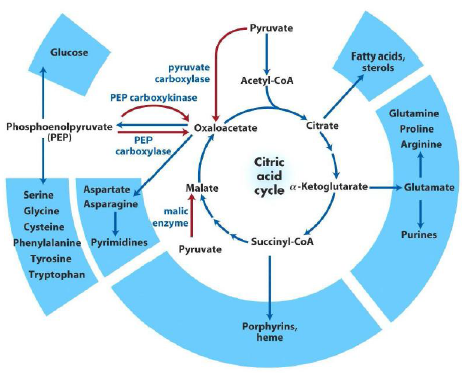
\includegraphics[width =8 cm]{Images/6.PNG} \\
        \textit{TCA cycle}     &   \textit{Anaplerosis} \\
        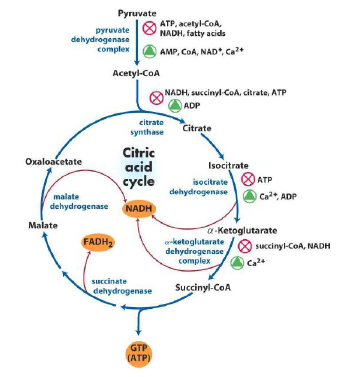
\includegraphics[width =8 cm]{Images/7.PNG}    & \\
        \textit{Régulation}    & \\
    \end{tabular}
\end{figure}


\noindent Le cycle de Krebs : gradient de protons accumulé et dissipé par une ATPases = couplage respiratoire \\

\mivbox{mivboxblue}{
cf Wikipédia \\
Réaction anaplérotique : qualifie une réaction chimique qui produit un métabolite, c'est-à-dire une espèce chimique intermédiaire d'une voie métabolique.

Anaplérose : consiste à rétablir la concentration des métabolites au sein du milieu mitochondrial afin qu'elle demeure constante et n'interrompe pas le cycle de Krebs malgré la consommation de ses métabolites par différentes biosynthèses ; élément essentiel de l'homéostasie cellulaire.

Réaction anaplérotiques majeures :
\begin{itemize}
    \item Pyruvate -(pyruvate carboxylase)-> Oxaloacétate
    \item Aspartate -(aspartate transaminase)-> Oxaloacétate
    \item Glutamate -(glutamate DH)-> $\alpha$-cétoglutarate
    \item $\beta$-oxydation des acides gras -(méthylmalonyl-CoA mutase)-> Succinyl-CoA
\end{itemize} 
}


\noindent De nombreuses enzymes sont régulées d'une manière allostériques, effecteur en lien avec la charge. 


\subsection{Méthodes pour étudier le métabolisme}

\begin{itemize}
    \item Métabolomique : identification et quantification des métabolites 
    \item Fluxomics : inférence ou prédiction du taux de réactions métaboliques dans les systèmes biologiques (cf Wikipedia)
    \item Outils analytiques basés sur :
        \begin{itemize}
            \item Résonance magnétique nucléaire (NMR)
            \item Spectrométrie de masse (MS)
            \item Chromatographie liquide (LC)
        \end{itemize}
\end{itemize}

\noindent Méthode de flux métabolique : vitesse réactionnelle lorsqu'il opère à l'état stationnaire

\begin{figure}[!h]
    \centering
    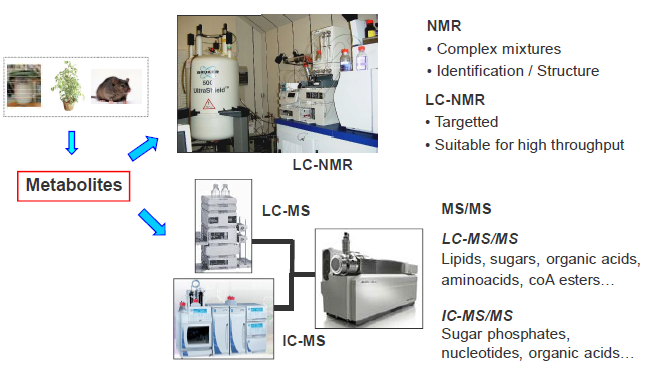
\includegraphics{Images/8.PNG}
    \caption{Métabolomique}
\end{figure}

\noindent La résonance magnétique nucléaire (NMR) permet une analyse structurale. C'est une méthode peu sensible : molarité > mm , il ne détecte que les métabolites présents en grande quantités.  

\noindent MS/MS : sépare selon la masse et permet d'identifier les produits de fragmentation.

\begin{figure}
    \centering
    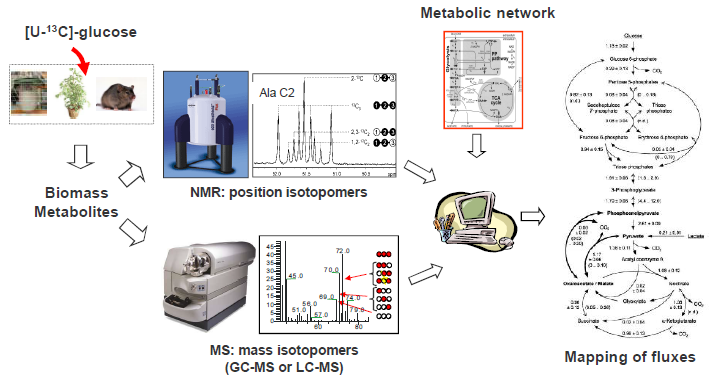
\includegraphics{Images/9.PNG}
    \caption{Flux measurements}
\end{figure}


\paragraph{}Il est plus difficile de chercher à mesurer les flux internes. La méthode de marquage des molécules ($^{13}C$, $^{15}N$) peut être utilisée. $\Rightarrow$ mesure la distribution des isotopomères des métabolites = distribution d'un marquage $\Rightarrow$ modèle

\paragraph{} Exemple :

Glucose marqué $\Rightarrow$ acide aminé marqué $\Rightarrow$ voie de biosynthèse connus

$\hookrightarrow$ modèle $\Rightarrow$ à partir de la distribution des isotopomères on peut représenter les flux

\mivbox{mivboxblue}{Isotopomères : }


\begin{figure}[!ht]
    \centering
    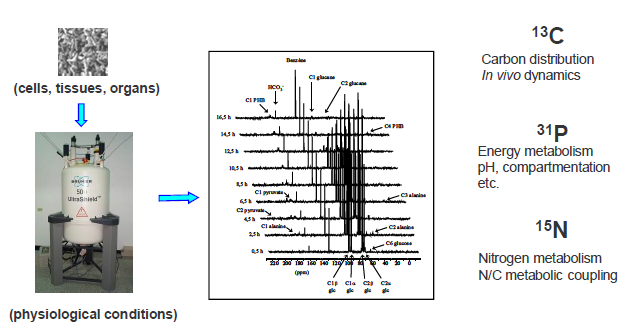
\includegraphics{Images/10.PNG}
    \caption{\textit{in vivo} NMR}
\end{figure}

\paragraph{}NMR peut être utilisé \textit{in vivo} uniquement si la molécule est majoritairement détectée.
$^3P$ : très utilme pour mesurer la charge énergétique, le pH


\subsection{Cinétique enzymatique : Michaelis-Menten}

Une \textbf{enzyme} est une protéine catalysant une réaction, elle facilite la réaction avec aucun changement de conformation.

$$E + S  \leftrightarrows ES \rightarrow E + P$$

\paragraph{}Action cinétique de la masse (Mass action kinetics) :
\begin{align*}
v_1 &=k_1E.S - k_{-1}ES\\
v_2 &=k_2ES
\end{align*}

\paragraph{}Quasi steady-state :
$$v_1=v_2=v$$
$$E + ES = E_0$$

\begin{align*}
&v = E_0 \frac{k_ES}{1+ \frac{S}{K_m}} \text{ taux de réaction } (M.s^{-1}) \\
&K_m = \frac{k_{-1}+k_{cat}}{k_1} \text{ Constance de Michaelis } (M)\\
&k_E =\frac{k_{cat}}{K_m} \text{ efficience catalytique } (M^{-1}.s^{-1})\\
&k_{cat} \text{ est le taux de turn-over maximal } (s^{-1})
\end{align*}

\paragraph{Michaelis-Menten Réversible}

$$E + S \leftrightarrows ES \leftrightarrows E + P$$

\begin{center}\fbox{$v=E_0 \frac{k_+S - k_-P}{1+ \frac{1}{K_S} + \frac{P}{K_P}}$}\end{center}
\noindent Il s'agit de l'\textcolor{red}{expression par défaut} pour la modélisation cinétique, équivalent quand $k_{-}=0$, parce qu'il explique le phénomène de competitive product inhibition.


\paragraph{Inhibition compétitive}
\begin{align*}
    E & + S 	\leftrightarrows ES \leftrightarrows & E + P \\
    \Updownarrow &  &  \Updownarrow \\
    E.I &  & E.I
\end{align*}



$$v = E_0 \frac{k_+S- k_-P}{1 + \frac{1}{K_S} + \frac{P}{K_P} + \frac{I}{K_{Ic}}}$$


\paragraph{Autres inhibitions}
\paragraph{}\noindent Non-compétitive (plus efficace à forte concentration en substrat)
$$v=E_0 \frac{k_+S-k_-P}{1+(\frac{S}{K_S}+\frac{P}{K_P})(1+\frac{I}{K_{Iu}})}$$


\noindent Mixed
$v=E_0 \frac{k_+S-k_-P}{1+(\frac{S}{K_S}+\frac{P}{K_P})(1+\frac{I}{K_{Iu}})+\frac{I}{K_{Ic}}}$




\paragraph{Multiples substrats et produits}
Si les substrats et les produits se lient indépendamment et dans un ordre aléatoire :

$$v=E_0\frac{k^+_{cat} \prod_{i} \frac{S_i}{K_{S_i}}-k^-_{cat} \prod_{j} \frac{P_j}{K_{P_j}}}{\prod_{i} (1+ \frac{S_i}{K_{S_i}}) + \prod_{j}(1+\frac{P_j}{K_{P_j}})-1}$$


\noindent source : 'Convenience kinetics' Liebermeister \& Klipp, 2006, Theoret. Biol. Med. Mod. 3:41




\paragraph{Relation de Haldane}
La contrainte de l'équilibre : $$K_{eq}=\frac{k^+_{cat} \prod_{j}K_{P_j}}{k^-_{cat} \prod_{i}K_{S_i}}$$


\paragraph{Cinétique enzymatique \& Thermodynamique}
Si on appelle $\Gamma$ le rapport de l'action de masse (mass action ratio) : $$ \Gamma = \frac{\prod_{j}P_j}{\prod_{i}S_i} = K_{eq}exp(\Delta G'/RT)$$

\noindent La cinétique enzymatique peut être divisée en 3 termes : $$v=k^+_{cat}E_0.f(S_i,P_j).(1-\Gamma/K_{eq})$$
\begin{itemize}
\item $1^{er}$ terme : $k^+_{cat}E_0$ correspond à la capacité enzymatique
\item $2^{nd}$ terme : $0 < f(S_i,P_j) < 1$ est le terme de saturation enzymatique. 
\textit{Comme un exercice, écrire ce terme pour la cinétique de Michaelis-Menten réversible}.
\item $3^{ème}$ terme : terme purement thermodynamique, il est indépendant des propriétés enzymatiques $\frac{1-\Gamma}{K_{eq}}=1-exp (\Delta G'/RT)$
\end{itemize}



\textbf{Cooperativity ?}
Equation de Hill : $$v=E_0 \frac{k_{cat}(S/K_{0.5})^h}{1+(S/K_{0.5})^h}$$

\noindent $h$ est le coefficient de Hill. Typiquement : $0.5<h<4$.
Cette équation est purement empirique (actuellement érronné pour $S<<K_{0.5}$).
$K_{0.5}$ est une constante phénoménologique (pas un $K_m$ !).

\paragraph{2-site cooperative binding}
Equation d'Adair :
$$v=2E_0k_{cat} \frac{S/K_1 + S^2 / K_1K_2}{1+2S/K_1+S^2/K_1K_2}$$
\noindent reastically captures site dependencies.

\paragraph{Saturation}
$E+S \leftrightarrows ES$
$E+ES=E_0$
$\frac{E.S}{ES}=\frac{k_{-1}}{k_1}=k_d$
$Y=\frac{ES}{E_0}=\frac{S/K_d}{1+S/K_d}$


\paragraph{Pour aller plus loin ...}
\begin{itemize}
\item \textit{Understanding the Control of Metabolism}, by David Fell, Portland Press, London, 1997
\item \textit{Fundamentals of Enzyme Kinetics}, by Athel Cornish-Bowden, Portland Press, London, 2004
\end{itemize}


\paragraph{Pour les TP :}
\begin{itemize}
\item The practical course will rely heavily on the theoretical course
\item Familiarize yourself with the COPASI modeling environment
http://www.copasi.org  (COPASI handbook)
\item  Refresh your course in linear algebra
\item Be prepared to use your favourite mathematical package
such as Octave, Scilab, Maple, R or Matlab
\item You will be evaluated on the practical course
\end{itemize}


\newpage
\renewcommand{\labelitemi}{$\bullet$}
\renewcommand{\labelitemii}{$\cdot$}
\renewcommand{\labelitemiii}{$\diamond$}
\renewcommand{\labelitemiv}{$\ast$}

\section{Introduction à la théorie du contrôle métabolique}

\paragraph{Outline}
\begin{itemize}
	\item Introduction à l'analyse de la sensibilité systémique
	\item Un exemple simple
	\item La matrice stœchiométrique
	\item L'évolution du système
	\item Les coefficients de contrôle
	\item \textit{Summation theorem}
	\item Coefficients de réponse et d'élasticité
	\item Théorème de connectivité
\end{itemize}


\paragraph{Problème général}
\begin{itemize}
	\item Prenons un \textcolor{blue}{réseau métabolique complexe arbitraire}
	\item Chaque vitesse de réaction répond au changements de concentrations en substrats, produits et quelque effecteurs :
	\begin{itemize}
		\item Ces lois cinétiques ont des \textcolor{blue}{propriétés moléculaires particulières}
	\end{itemize}
	\item Questions importantes du MCT :
	\begin{itemize}
		\item Comment le système réponds aux changements des propriétés moléculaire individuelle (activités des enzymes) ?
		\item Comment la réponse du système dépend de la \textcolor{blue}{structure du réseau} ?
		\item Comment sont contraintes les sensibilités systémiques ? Est-ce qu'elles montrent des dépendances ?
	\end{itemize}
\end{itemize}
\textit{Quelles répercutions au systèmes entier par rapport aux propriétés individuelles ?}


\paragraph{État stationnaire et définition du système}
Le métabolisme est une usine chimique, une fonction durable pour traiter les nutriments et produire de la biomasse, énergie, déchets, etc. Il doit atteindre un \textbf{état stationnaire stable} (contrainte).

Donc :
\begin{itemize}
	\item Le système \textbf{doit être ouvert} afin d'atteindre un état stationnaire non-trivial réalisable thermodynamiquement (i.e, avec des flux non-nuls).
	\item La plupart des réactions doivent être sensible à la concentration des substrats et des produits, permettant la balance de la production de métabolites et des taux de consommations (équilibre entre flux entrants et sortant).   	
\end{itemize}


\paragraph{Raisonnement intuitif ?}
\begin{figure}
	\centering
	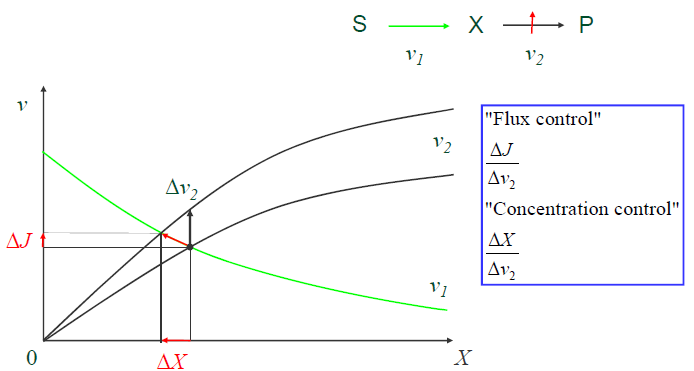
\includegraphics{Images/02_1.PNG}
\end{figure}
$X$ est un métabolite intermédiaire. L'état stationnaire est atteint  lorsque $v_1 = v_2$ = intersection des deux courbes. 
Le changement de flux dans ce cas est plus petit que le changement de vitesse de la seconde réaction. 


\paragraph{Quantitativement ?}
\begin{figure}
	\centering
	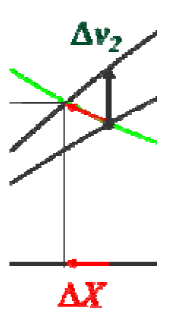
\includegraphics{Images/02_2.PNG}
\end{figure}
Prenons $E_2$ l'activité de l'enzyme 2. A l'état stationnaire :
$$ v_1(X,E_1) = v_2(X,E_2) $$
$$ \frac{\partial v_1}{\partial x} \Delta X \simeq \frac{\partial v_2}{\partial x} \Delta X + \frac{\partial v_2}{\partial E_2} \Delta E_2 $$

à la limite :
\textbf{Contrôle de la concentration} : \fbox{$\frac{\partial X}{\partial E_2} = \frac{-1}{\frac{\partial v_2}{\partial x}- \frac{\partial v_1}{\partial x}} $}
si $v_2$ et $E_2$ sont exprimés dans les mêmes unités. 


\paragraph{Quantitativement ?}
\begin{figure}
	\centering
	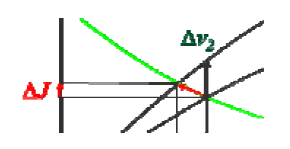
\includegraphics{Images/02_3.PNG}
\end{figure}
$$ J=v_2(X,E_2) $$
$$ \Delta \simeq \frac{\partial v_2}{\partial x} \Delta X + \frac{\partial v_2}{\partial E_2} \Delta E_2 $$

à la limite :
\textbf{Contrôle du flux} : \fbox{$\frac{\partial J}{\partial E_2} = \frac{\frac{\partial v_1}{\partial x}}{\frac{\partial v_2}{\partial x}- \frac{\partial v_1}{\partial x}} $}


\paragraph{Quantitativement ?}
Si nous modulons $E_1$ on obtient de manière similaire :

\fbox{	$  \frac{\partial X}{\partial E_1} = \frac{1}{\frac{\partial v_2}{\partial x}- \frac{\partial v_1}{\partial x}} $
$\frac{\partial J}{\partial E_1} = \frac{\frac{\partial v_2}{\partial x}}{\frac{\partial v_2}{\partial x}- \frac{\partial v_1}{\partial x}} $ }

Le contrôle du flux par l'apport de la réaction 1 est proportionnel à la sensibilité .........
\textit{Flux control by supply reaction 1 is proportional to sensitivity of demand reaction 2 to intermediate metabolite}


\paragraph{Quantitativement ?}
et nous obtenons la \textbf{relation de sommation} suivante : 
\fbox{ $ \frac{\partial X}{\partial E_1} + \frac{\partial X}{\partial E_2} = 0 $}
\fbox{$ \frac{\partial J}{\partial E_1} + \frac{\partial J}{\partial E_2} = 1 $ }

Contrôle de la concentration selon l'offre et la demande : signes opposés
Concentration control by supply and demand of opposite signs

Contrôle du flux selon l'offre et la deande ...
Flux control by supply and demand add up to 1


\paragraph{Plus généralement}
Il est possible d'obtenir un traitement général de la théorie du contrôle du système métabolique de \textbf{complexité arbitraire}. \textit{C. Reder (1988) J. Theoret. Biol. 135:175-201} 

\textbf{Définitions générales}:
\begin{tabular}{ll}
	$x = x(t,p)$ 	&	vecteur de concentrations, fonction du temps et des paramètres \\
	$X = X(p)$ 	&	vecteur de concentrations à l'\textbf{état stationnaire} : $dx/dt=0$ \\
	$v=v(x,p)$	&	vecteur des vitesse, fonction des molarités et des paramètres (\textit{expression inétique du système}) \\
	$J=J(p) = v(X(p),p)$	&	vecteur de flux à \textbf{l'état stationnaire}
\end{tabular}


\paragraph{La matrice stœchiométrique $N$}
\begin{itemize}
	\item Les réactions du réseau sont exprimés dans la matrice stœchiométrique $N$, où les colonne continnent les coefficients stœchiométriques de chaque réaction.
	\item Cette matrice reflète la \textbf{structure du système}
	\item N est de rang maximal si et seulement s'il n'y a pas de relation de conservation contraignant les différentes concentrations, que nous allons supposer initialement pour simplifier
	\item Sinon, elle peut être réduite à une matrice $N^0$ avec un rang maximal afin de traiter avec des variables indépendantes : $$ N=L.N^0 $$
\end{itemize}


\paragraph{Évolution du système}
L'évolution du vecteur de concentration $x$ du système est une fonction simple du vecteur de vitesse $v$ :

\fbox{ $ \frac{dx}{dt}=N.v(x,p)$} où $p$ est un vecteur de paramètres, incluant l'activité des enzymes.

La Jacobienne est :	$$ \textswab{J}  = N. \frac{ \partial v}{\partial x}     $$

$\frac{\partial v_i}{\partial x_j} $ : 'élasticités' non-normalisées


\paragraph{Contraintes des flux à l'état stationnaire}
Nous sommes intéressé par l'analyse de l'état stationnaire du système :
		$$ dx/dt = N . v(X(p),p) = 0 $$
où $X(p)$ est le vecteur des concentrations à l'état stationnaire.

L'état stationnaire introduit des \textbf{dépendances linéaires} entre les flux : 
$$ N. J(p) = 0 $$
Loi de Kirchhoff pour les métabolites intermédiaires 

Donc le vecteur de flux $J$ peut être exprimés dans la base de $Ker(N)$ (souvent appelé $K$) 


\paragraph{Contrôle de l'expression systémique}

Faisons la différence entre l'équation de l'état d'équilibre par rapport à $p$ :
$$ N . \frac{\partial v}{\partial x} . \frac{ \partial X}{\partial p} + N . \frac{\partial v}{\partial p} = 0 $$
\fbox{$ \frac{\partial X}{\partial p} = - (N. \frac{\partial v}{\partial x})^{-1} . N . \frac{\partial v}{\partial p} $}

\fbox{$ \frac{\partial X}{\partial p} = - \textswab{J}^{-1} . N . \frac{\partial v}{\partial p} $}

Cette équation relie les \textbf{changements systémiques} dans l'état stationnaire des concentrations $X$ aux changements de vitesse $v$.

La matrice $ \Gamma = - (N. \frac{\partial v}{\partial x})^{-1} . N  = - \textswab{J}^{-1} . N $ contient tous les \textbf{coefficient de contrôle des concentrations}.


\paragraph{Contrôle des flux}
Let us calculate the resulting steady-state flux : (MAL DIT) 
	$$ J=c(X(p),p) $$
and differentiate it respect to $p$ :
\begin{align*}
	\partial J / \partial p & = \partial v / \partial x . \partial X / \partial p + \partial v / \partial p \\
							& = ( \partial v / \partial x . \Gamma + I ) . \partial v/ \partial p 
\end{align*}

Cette équation relie les changements systémiques dans l'état stationnaire des flux $J$ aux changements de vitesses $v$.

La matrice $ \Phi = I + \partial v / \partial x . \Gamma $ contient tous les \textbf{coefficients de contrôle du flux}. 



\paragraph{Généralisation}
Si le système montre des \textbf{relations de conservation} comme $[ATP]+[ADP]+[AMP] = constante$, nous devons réduire la matrice $N$ à la matrice $N^0$ avec un rang maximal correspondant à une molarité des métabolites indépendants $x^0$.
\begin{align*}
	N & = L. N^0 \\
	dx^0/dt &= N^0 . v(x,p) \\
	\textswab{J} &= N^0 . \partial v / \partial x . L \\
	\Gamma & = - L . \textswab{J} ^{-1} . N^0 \\
	\Phi = I + \partial v / \partial x . \Gamma
\end{align*}




\paragraph{Coefficients de contrôle normalisé}

Il est de coutume d'exprimer le contrôle en termes de coefficients de contrôle \textbf{normalisés} sans dimension :

\begin{tabular}{rr}
	Contrôle du flux	&	$C_i^j = \frac{E_i}{J_j} \frac{\partial J_j}{\partial E_i } = \frac{\partial ln J_j}{\partial ln E_i}$ \\
	Contrôle des concentrations	&	$C_i^{X_j} = \frac{E_i}{X_j} \frac{\partial X_j}{\partial E_i } = \frac{\partial ln X_j}{\partial ln E_i}	$ \\
\end{tabular}

où les paramètres $E_i$ dénote les \textbf{activités enzymatiques}, en général exprimé dans les mêmes unités que $J_i (M.s^{-1})$.


\newpage
\renewcommand{\labelitemi}{$\bullet$}
\renewcommand{\labelitemii}{$\cdot$}
\renewcommand{\labelitemiii}{$\diamond$}
\renewcommand{\labelitemiv}{$\ast$}

\section{Cours 7 octobre}

Le système métabolique fonctionne à l'état stationnaire. L'équation de l'état stationnaire est : $$N.v(X,E) = 0$$ est \textbf{invariant à une graduation arbitraire} des activités de E.

Équivalent à considérer ce qui se passe lorsque l'on multiplie par un même facteur arbitraire positif (multiplier toutes les activités par le même facteur).

De manière générale, revient à multiplier la fonction v (x,E) par ce facteur alpha
$$ v(X,\alpha E) = \alpha v(X,E)  \forall \alpha \in \mathbb{R}^+ $$
par voie de conséquence on à N.v(X,E) = 0
==> invariante par ce genre de modification

==> Lorsque l'on fait cette modification, on est toujours à l'état stationnaire

Résultat: toutes les vitesses réactionnelles sont multipliées par ce facteur alpha = tous les flux sont multipliés par ce facteur alpha.

Par conséquent, le vecteur de flux $J$ est une fonction homogène de $1^{er}$ ordre de l'activité de l'enzyme E : 
$$J(\alpha E) = \alpha J(E), \text{.....}  \forall \alpha \in \mathbb{R}^+ $$
et les concentrations $X$ sont des fonctions homogène d'ordre 0 :
$$ X(\alpha E) = X(E), \text{.....}  \forall \alpha \in \mathbb{R}^+ $$
 
 
 
 

\textit{$f(\alpha x = \alpha ^n f(x)$  avec $n=$ ordre de la fonction homogène }
$X(\alpha E) = X(E)$

Point technique concernant les fonction homogène : dérivation des fonctions homogènes :
$$f(\alpha x) = \alpha ^n f(x)$$

$$	\sum \frac{df}{dx_i} x_i = n \alpha ^{n-1} f(x)$$

\fbox{$\sum \frac{df}{dx_i} x_i = n f(x)$} 




\section{Summation relationship - Relation de sommation}

Les théorèmes de sommation suivent directement par dérivation en ce qui concerne $\alpha$ :  \fbox{MAL DIT}

Pour les flux, J fonction homogène d'ordre 1  de E : 

$$ \sum_i \frac{ \partial Jj}{\partial E_i}E_i = J_j$$ 
$$ \sum_i \frac{\partial J_j}{\partial E_i} \frac{E_i}{J_j}=1 $$
J est un vecteur => peut être écrite pour toutes les composantes j

$$\frac{\partial J_j}{\partial E_i}\frac{E_i}{J_j}  \Rightarrow  C_i^j $$
relation qui lie toutes les coefficients de contrôle du flux $j$ et leurs somme est égal à :
$$	\sum_i \frac{\partial J_j}{\partial E_i}\frac{E_i}{J_j} \Rightarrow \sum_i C_i^j $$
Le contrôle du flux est \textbf{distribué} à travers le système.


Pour les concentrations, le vecteur des concentrations $X$ à l'état stationnaire est une fonction homogène d'ordre 0 :
\fbox{$\sum_i C_i^{X_j}=0$}


$$ \sum_i \frac{dX_i}{dE_i}E_i = 0 $$
$$ \sum_i \frac{dX_j}{dEi} \frac{E_i}{X_j}=0 $$
Le coefficient de contrôle des concentration dans la variantes normalisées
$$ \frac{dX_j}{dEi} \frac{E_i}{X_j} = C_j^{X_j} $$
==> théorème de sommation


\section{Les coefficients de réponse}
La réponse linéarisée (LINEAIRE ?) du système à un changement de n'importe quel paramètre $p_i$ peut être exprimé à partir des coefficients de contrôle et des coefficients d'élasticité :

$$ R_i^j = \frac{p_i}{J_j} \frac{ \partial J_j}{\partial p_i} = \frac{p_i}{J_j} \sum_k \frac{\partial J_j}{\partial E_k} \frac{\partial v_k}{\partial p_i} 
		= \sum_k C_k^j \epsilon_i^k $$  où  $\epsilon_i^k = \frac{p_i}{v_k}\frac{\partial v_k}{\partial p_i} $

sont des coefficients d'élasticité normalisées exprimant les sensibilités des taux de modifications des paramètres.

Le $R_i^j$ sont appelés \textbf{coefficients de réponse}.


$$ R_i^j = \sum_k C_k^j \epsilon_i^k $$
La réponse du réseau dépend de deux facteurs :
\begin{itemize}
	\item Les sensibilités des enzymes aux paramètres $p_i$ (propriété moléculaire)
	\item La contrôle exercé par ces enzymes sur le flux (propriétés systémiques)
\end{itemize}

On peut de similairement définir des coefficients de réponse pour les concentrations en métabolite :
$$ R_i^{X_j} = \sum_k C_k^{X_j} \epsilon_i^k $$


\textit{Interprétation des relations : }
Multiplier l'activité par un même facteur alpha :

le coefficient de contrôle $\sum_i C_i^j$  multiplié par :
 si un facteur $\alpha proche$ de 1, 
on suppose que l'on change une activité i, pr def du coefficient de contrôle le changement relatif de 
	$$\frac{\delta J_j}{J_j} \simeq C_i^j \frac{\delta E_i}{E_i}$$
	$$ \simeq \sum C_i^j \frac{\delta E_i}{E_i} = \sum _i C_i^j (\alpha - 1) $$
	$$ E_i + \delta E_i = \alpha E_i $$
	$$ \delta E_i = (\alpha -1 ) E_i $$
			 	
 	==> on a le même changement relatif
 	
 	ici on utilise des coefficients de contrôle normalisés : si = 1 , 
 	=0 l'activité à aucun contrôle sur le flux
 	Le contrôle d'un flux va être distribué entre les différents flux du système.
 	
 	Le contrôle du flux va être distribué et cela se manifeste dans cette relation. 
 	==> il faut agir sur toute les activités.
 	
 	Le coefficient de contrôle peut être faible mais le contrôle du flux est distribué
 	
 	


\paragraph{Les relations de connectivité}

On peut exprimer la réponse d'un système à de petits changements avec les coefficient de contrôle. 
Calculer un coefficient de réponse du système à cette drogue :

coefficient de réponse = dérivé du flux par rapport aux paramètres dans sa version normalisée

avantage de normalisé (NORMEE ?) : grandeur sans dimension, =1 flux répond complètement à la drogue, = 0 flux insensible à la drogue

La dérivé peut être calculée en considérant toutes les activités enzymatiques du système :
$$ J_j = J_j(E_k(P_i)) $$



\paragraph{Question} 
coefficient de contrôle :	(mince ...) 
coefficient d'élasticité : comment influx sur l'activité de l'enzyme

Le flux est influencé par toutes les activités enzymatiques, chaque activité dépend de paramètres.

Propriété moléculaire des enzymes où les vitesses réactionnelles sont fonction des concentrations ($\frac{dv}{dx}$)

État stationnaire : la concentration est une variable qui dépend des paramètres et des activités

Le flux $J = v[X(E),E]$, J est une fonction des activités enzymatiques uniquement mais pas une fonction des concentrations. 
 	
$$ J_j = J_j(E_k(P_i))$$
$$ \frac{J_j}{P_i}= \sum_k \frac{dJ_j}{dE_k} \frac{dE_k}{d_pi} $$
$$ \Rightarrow \frac{dE_k}{d_pi}\text{ = sensibilité des enzymes aux paramètres }$$


$$ R^j_i = \sum_k \frac{Ek}{J_j}\frac{dJ_j}{dE_k}\frac{P_i}{E_k}\frac{dv_k}{dp_i}  $$

corr $\frac{P_i}{E_k}\frac{dv_k}{dp_i}$ dérivé d'une activité par rapport aux paramètres dans sa valeur normée = élasticité entre -1 et +1 (rarement en dehors) = sensibilité de l'activité aux paramètres 

$\Rightarrow$ définition d'élasticité, sensibilité d'une vitesse réactionnelle ou d'une activité et cela correspond à un paramètre

Elasticité = 1 : stimule l'activité, =-1 : inhibe l'activité, plus faible : faible inhibition ou stimulation


\textbf{Exemple :}
$$ v = v(x_i, E) = E f(x) \text{(pté d'homogénéité)} $$
 en faisant intervenir une droque $p$ (variable supplémentaire) :
	$$ v = v(x_i, E, p) $$
Par définition, l'élasticité $\epsilon_p^v = \frac{p}{v} \frac{dv}{dp}$, on a les paramètres $E$ et $P$, on peut définir une sensibilité de la vitesse réactionnelle :
	$$ \epsilon_E^v = \frac{E}{v}\frac{dv}{dE}=1 $$

Donc ici (diapo), plus précis d'écrire :
	$$ \frac{dJ_j}{dE_k}\frac{dE_k}{dv_k}\frac{dv_k}{dp_i} $$
	
\begin{tabular}{c|c|c}
	$\frac{Ek}{J_j} \frac{dJ_j}{dE_k}$	&	$\frac{v_k}{E_k}\frac{dE_k}{dv_k}$	&	$\frac{p_i}{v_k}\frac{dv_k}{dp_i}$ \\
	$\rightarrow$ coefficient de contrôle	&	$\rightarrow =  1$	&	$ = \epsilon$ \\
\end{tabular} 



$R_i^j$ : coefficient de réponse = somme des termes qui font intervenir les coefficients de contrôle et les sensibilités individuelles des enzymes aux paramètres (il faut une élasticité suffisante $+$ une enzyme cible de la drogue et un contrôle sur le système)

$\Rightarrow$ il permet de quantifier la réponse d'un système à une perturbation.

Pour réponse significative : cible(s) soient sensible(s) + dites cibles aient un contrôle sur le système




\section{Les relations de connectivité}
Théorème de connectivité : et en relation les coefficients de contrôle et les élasticités

$$\Gamma = -L . \textgoth{J}^{-1}.N^0 $$
$$ \Rightarrow \Gamma . \frac{\partial v}{\partial x} . L = - L $$


$dv/dx$ : réactivité du système à ce changement

La matrice de lien permet de passer de la matrice $N^0$ à la matrice de stœchiométrique complète $N$.

permet de dérire $\frac{dx}{dx^0}= L= (\frac{I}{roooooh})$ (matrice)
	$$ \frac{dx^0}{dt}= N^0v $$
	$$ \textgoth{J} = N^0 \frac{dv}{dx}L $$

$\Gamma$ : multiplié par $dv/dx$, lorsque toutes les variables sont indépendantes, la matrice de lien = matrice identité


$$ \Phi = I + \frac{\partial v}{\partial x} . \Gamma $$
$$ \Rightarrow    \Phi . \frac{\partial v}{\partial x} . L = 0 $$


$\phi$ : 
==> manière d'exprimer les relations


\paragraph{Les relations de connectivité}
Lorsque l'on utilise des élasticités normalisées, les relations de connectivité peuvent être exprimés avec les variables indépendantes $x_i^0$ :
$$ \epsilon_i^k = \frac{x_i^0}{v_k} \frac{\partial v_k}{\partial x_i^0} $$

\begin{equation}
   \fbox{$
   \begin{array}{rcl}
      \sum_k C_k^{X_j} \epsilon_i^k & = & - \delta_{ij} \\
      \sum_k C_k^j \epsilon_i^k & = & 0
   \end{array}
   $}
\end{equation}

où $\delta_{ij}$ est le coefficients de Kronecker :  $\delta_{ij} = 1\text{ if } i  = j $
et $\delta_{ij} = 0 \text{ if }i  \neq  j $



\paragraph{Les relations de connectivités}
$$ \sum_k C_k^{X_j} \epsilon _i^k  =  - \delta_{ij} $$
$$ \sum_k C_k^j \epsilon_i^k  =  0 $$
Ces relations peuvent être interprétées en terme de \textbf{réponse du système interne} à la perturbation $x_i^0$.

Ils sont nécessaire à la \textbf{stabilité du système} :
\begin{itemize}
	\item Le système contre/empêche les fluctuations de $x_i^0$
	\item Le reste du système est insensible à ces fluctuations à l'approximation du $1^{er}$ ordre
\end{itemize}





\paragraph{Explications}
Dans le cas d'une matrice de rang maximum :
$$ \Gamma \frac{dv}{dx}= -I $$
$ \sum C_k^{X_j}\frac{dv_k}{dX_i}= $	\textbf{-1} (terme diagonaux si $i=j$) \textbf{ou} 	\textbf{0} si $i \neq j$

k = réaction donc une activité, 

\textbf{flux}: pour une réaction k, vitesse réactionnelle et définir un flux dépend des paramètres et qui correspond à la vitesse des paramètres obtenus à l'état stationnaire

$C_k^j$ : $j$ une réaction enzymatique et $j$ le flux cible

$C_k^{X_j}$ : une réaction qui contrôle la concentration $j$ (mal dit)

Dans le cas des coefficient de réponse : réponse à un paramètre extérieur alors que dans T connectivité :  à des changements internes (concentration d'un métabolites particulier)
==> interprétation physique

Relation : exprimant la réponse du système à des fluctuations sur les temps, au premier ordre, la répercution sur le reste du système va être nu à l'exception de la réponse de $X_i$ à ces propres fluctuations => ces relations sont nécessaire pour la stabilité du système

Stabilité: valeur propres jacobienne

Ce que l'on interprète : le système à l'état stationnaire réagit aux fluctuations sur les temps et il a tendance à contré les fluctuations. Si fluctuation d'une concentration, il contre la fluctuation. 



\paragraph{Résumé de la séance :}
\begin{itemize}
	\item La réponse du système dépend à la fois des propriétés individuelles des enzymes du système et de la structure du système. On est capable de séparer les deux.
	

	\item \textbf{Les flux métaboliques sont contraints} à une faible dimension dans le sous-espace parce que le pool de métabolites  s'équilibre à l'état stationnaire
	\begin{itemize}
		\item Les flux métaboliques sont contraints par la condition de stationnarité. Cette contrainte correspond à la condition que les pulls métaboliques n'évoluent plus (somme entrant = somme sortant), beaucoup moins de flux indépendant que de arg
	\end{itemize}
	
	
	\item Le contrôle du flux est généralement \textbf{distribué} à travers le système (pas de 'bottleneck')
	\begin{itemize}
		\item C'est important pour la biotechnologie et la pharmacologie
		\item un bottleneck, une réaction qui contrôle tout un flux est rare, le flux est distribué.  Ex: augmenter un produit, nécessite de toucher à plusieurs enzymes
	\end{itemize}

	\item Le comportement du système peut être considéré sous un principe général d'\textbf{action-réaction} :
	\begin{itemize}
		\item Il tamponne généralement les changements imposés de l'extérieur
		\item Il neutralise les fluctuations internes
		\item \textit{Notion de coefficient de contrôle, action = réagit sur activité enzymatique, et réaction = résultat moindre que celui attendu après l'action.}
	\end{itemize}
\end{itemize}


\newpage
\renewcommand{\labelitemi}{$\bullet$}
\renewcommand{\labelitemii}{$\cdot$}
\renewcommand{\labelitemiii}{$\diamond$}
\renewcommand{\labelitemiv}{$\ast$}

\section{cours 3 - Simon}

\paragraph{}Aujourd'hui on va voir deux théorèmes très généraux qui lient ces coefficients de contrôle.
\begin{enumerate}
\item théorème sur la somme des coefficients de contrôle;
\item théorème de connectivité qui associe les coefficients de contrôle et les elasticités.
\end{enumerate}

\subsection{Théorème sur la somme}

\paragraph{}On part toujours de l'équation de base qui est celle qui écrit que le système métabolique fonctionne à l'état stationnaire (maintenant vous devez avoir l'habitude de cette équation):
$$N.v(X,E)=0$$
Un point particulièrement important à noter sur cette équation c'est de considérer ce qui se passe lorsque l'on multiplie toutes les activités par un même facteur $\alpha$ connu. Vous voyez l'idée ? C'est qu'on a un système métabolique à l'état stationnaire et puis on se demande ce qu'il se passe si on multiplie toutes les activités de tous les enzymes par le même facteur. \\
De manière générale, cela revient à multiplier la fonction $v(X,E)$ par ce facteur $\alpha$. Cela veut simplement dire que la vitesse réactionnelle est proportionnelle à l'activité de l'enzyme. Donc on a :
$$v(x,\alpha E) = \alpha v(X,E)$$
Pour rappel $E$ est le vecteur qui contient toutes les activités des enzymes. Ce que l'on remarque c'est que par voie de conséquence on a 
$$N.v(X,\alpha E)=0$$
Donc le point important c'est que l'équation de stationnarité est invariante par rapport à ce genre de transformation qui consiste à multiplier toutes les activités par le même facteur.\\
Lorsqu'on fait cette opération, on est toujours en état stationnaire et donc les concentrations des métabolites à l'état stationnaire restent inchangés. Puisque le même vecteur $X$ est la solution à la fois de $N.v(X,E)=0$ et de $\alpha N.v(X,E)=0$.\\
D'une part toutes les vitesses réactionnelles sont multipliées par ce facteur $\alpha$, donc le flux est multiplié par ce facteur $\alpha$, donc le vecteur de flux est une fonction homogène du premier ordre des activités. C'est à dire que :
$$J(\alpha E) = \alpha J(E)$$

\mivbox{mivboxgreen}{Je ne sais pas si vous êtes familiers avec les fonctions homogènes mais une fonction homogène tel que :
$$f(\alpha x) = \alpha^{n}f(x)$$
$n$ c'est l'ordre de la fonction homogène.
}

\paragraph{}Donc ici on a le flux qui est une fonction homogène du premier ordre des activités et puis puisque les concentrations ne bougent pas, elle sont aussi une fonction homogène d'ordre 0 des activités.
$$X(\alpha E) = X(E)$$
Et ceci quel que soit le facteur $\alpha$ par lequel on multiplie toutes les activités du système.\\

\mivbox{mivboxgreen}{
Un point technique qui va nous être utile concernant les fonctions homogènes concerne la dérivation des fonction homogènes. Donc ici on va prendre le cas général où f est une fonction vectorielle d'un vecteur x. On peut dériver cette expression par rapport à $\alpha$. Donc on fait :
$$\sum{\frac{\partial f}{\partial x_{i}}x_{i}}=n \alpha^{n-1}f(x)$$
\textit{En français : somme de df sur toutes les composantes du vecteur $x$ et ensuite dériver chaque terme $\alpha x_{i}$ par rapport à $\alpha$, c'est à dire que ce sera multiplié par $x_{i}$... en dérivant le terme de gauche par rapport à $\alpha$ et à droite on a tout simplement n $\alpha$ puissance $n-1$ $f(x)$.}\\
Et comme je disais ces expressions sont valables quelque soit la valeur de $\alpha$ donc on peut prendre par exemple $\alpha=1$ et on a donc l'expression remarquable qui est :
$$\sum{\frac{\partial f}{\partial x_{i}}x_{i}}=n f(x)$$
Donc ça c'est une propriété des fonctions homogènes pour dériver une fonction homogène par rapport à ... on verra par la suite ... qui lie les dérivés premières. Ce qui apparaît ici, c'est l'ordre de la fonction homogène : le $n$ à droite.
}
\paragraph{}On va utiliser directement cette gymnastique sur les fonctions homogènes et on va voir ce que ça va nous donner.\\
Donc voilà l'exercice! Je vous rappelle on avait par exemple\\
\begin{center}$J = $ fonction homogène d'ordre 1 des activités ($E$)\end{center}
Et donc :
$$\sum_{i}{\frac{\partial J_{i}}{\partial E_{i}}E_{i}=N J_{j}} \text{\qquad , où $N$ vaut 1}$$
Donc $J$ je vous rappelle c'est un vecteur et donc on peut l'écrire pour toutes les composantes du vecteur par exemple pour la composante particulière $_{j}$.\\
On peut diviser à gauche et à droite par le flux que l'on considère non nul pour un système métabolique qui fonctionne avec un flux non nul. Donc on a :
$$\sum_{i}{\frac{\partial J_{j}}{\partial E_{i}}\frac{E_{i}}{J_{j}} = 1}$$
Donc ce 1, c'est l'ordre de la fonction homogène. Ce qu'on reconnaît dans la somme c'est précisément ce dont j'avais introduit la définition il y a quelques minutes, c'est le coefficient de contrôle du flux $J$ par la réaction $_{i}$ dans sa version normalisée, notée $C_{i}^{j}$.\\
Donc on est bien arrivé à un résultat remarquable où on a une relation qui lie tous les coefficients de contrôle du flux $J$ et leur somme est égale identiquement à 1.\\
Après on viendra sur l'interprétation de cette relation de sommation mais si on continue exactement de la même manière sur les concentrations on a :

\begin{center} Vecteur des concentrations à l'état stationnaire = fonction homogène d'ordre 0 des activités
\end{center}

Donc ça se décline exactement pareil :
$$\sum_{i}{\frac{\partial X_{j}}{\partial E_{i}}E_{i} = 0}$$
On peut tout aussi bien diviser tous les termes de la somme par $X_{j}$ et donc on a :
$$\sum_{i}{\frac{\partial X_{j}}{\partial E_{i}}\frac{E_{i}}{X_{j}} = 0}$$
Et à gauche, on reconnaît les coefficients de contrôle de concentrations dans la version normalisée : $C_{i}^{X_{j}}$\\
Ce qui veut dire que la somme des coefficients de contrôle sur toutes les activités $_{i}$ sur un métabolique particulier $_{j}$ est identiquement nulle : $\sum_{i}{C_{i}^{X_{j}}}=0$\\

\paragraph{}Comment va t-on interpréter ces relations ? Précisément, elles ont à voir avec l'expérience par la pensée que je mentionnais tout à l'heure qui consiste à multiplier toutes les activités par un facteur $\alpha$. Par définition du coefficient de contrôle :
$$\frac{\delta J_{j}}{J_{j}} \sim C_{i}^{j}\frac{\delta E_{i}}{E_{i}}$$
\textit{En français : le changement relatif delta Jj sur Jj est asymptotiquement égale au coefficient de contrôle Cij que multiplie le changement d'activité delta Ei sur Ei}

\paragraph{}De manière plus générale, par linéarité, on a :
$$\frac{\delta J_{j}}{J_{j}} \sim \sum{C_{}^{}\frac{\delta E_{i}}{E_{i}}}$$
\textit{En français : delta Jj qui est asymptotiquement égale à la somme des produits des coefficients de contrôle que multiplie les changement relatifs des différentes activités}

\paragraph{}Lorsque tous ces changements relatifs sont égaux, c'est à dire qu'on écrit (on avait multiplié par $\alpha$ donc on a) :
$$E_{i} + \delta E_{i} = \alpha E_{i}$$
$$\delta E_{i} = (\alpha - 1) E_{i}$$
Donc si tous les changements ont le même facteur de proportionnalité, donc ce qu'on avait [19min47 B01]


\newpage
% \textswab{J}

\renewcommand{\labelitemi}{$\bullet$}
\renewcommand{\labelitemii}{$\cdot$}
\renewcommand{\labelitemiii}{$\diamond$}
\renewcommand{\labelitemiv}{$\ast$}

\section{Cours X  Amorce pour l'analyse de stabilité : Analyse de la stabilité des systèmes métaboliques}

\paragraph{La Jacobienne $\textswab{J}$ d'un système différentiel}
Considérons un système d'équation différentielles ordinaires (ODEs) : 
$$ dx/dt = f(x) $$
Nous définissons sa matrice Jacobienne comme la matrice de ses dérivées partielles :
$$ \textswab{J} = \partial f / \partial x $$
qui est une matrice carré.


\paragraph{Évolution du système autour de l'état stationnaire}
Considérons maintenant le système autour d'un état stationnaire $X$ :
$$ dx/dt(X) = f(X)=0$$
Dans le voisinage de $X$, nous pouvons utiliser l'approximation de premier ordre
$$ dx/dt \sim \textswab{J} . [x-X] $$
qui intègre dans
$$ x-X = exp( \textswab{J}t) . [x(0)-X] $$
en utilisant la matrice exponentielle
$$ exp( \textswab{J}t) = \sum_{k=0}^{\inf} \frac{1}{k!} \textswab{J}^k t^k $$



\paragraph{Conditions de stabilité autour de l'état stationnaire}
Considérons les valeurs propres $\lambda_i$ de la matrice Jacobienne, 

L'état stationnaire est instable si : $$ \exists_i, Re(\lambda_i)>0 $$

L'état stationnaire est exponentiellement stable \fbox{MAL DIT} si : $$ \exists_i, Re(\lambda_i)<0 $$

avec un temps de relaxation $\tau_i = \frac{1}{|Re(\lambda_i)|}$ 
et une fréquence $ \omega_i = \frac{|Im(\lambda_i)|}{2\pi} $



\paragraph{Bifurcations}
Considérons les valeurs propres $\lambda_i(p)$ de la matrice Jacobienne quand les paramètres varient.

Un bifurcation nœud-selle correspond au passage par zéro d'une valeur propre réelle $\lambda_i$

Une bifurcation de Hopf correspond à un passage par zéro de la partie réelle $Re(\lambda_i)$ d'une paire de valeurs propres conjuguées $ Re(\lambda_i) \pm 2i\pi\omega_j $

Il existe plusieurs autres types de bifurcation plus complexes.



\paragraph{Jacobienne d'un système métabolique}
A partir de l'équation d'évolution 
$$dx/dt = N . v(x,p) $$
nous dérivons la Jacobienne 
$$ \textswab{J} = N. \partial v / \partial x $$


Cependant cette Jacobienne est singulière si $N$ n'est pas de rang maximal. Il est alors utile de réduire le système à des variables indépendantes :
\begin{tabular}{lc}
			&	$dx^0/dt = N^0 . v(x,p)$ \\
	with	&	$N=L.N^0$	\\
			&	$\partial x / \partial x^0=L $
\end{tabular}
et nous dérivons la Jacobienne :
$$ \textswab{J}=N^0 . \partial v / \partial x . L $$
qui doit être définie négative pour que le système soit stable.



\end{document}
